

\subsection{Dynamic Prior Selection in Bayesian Inference}
A potential improvement in Bayesian modeling is the use of dynamically selected priors instead of static priors. This could be achieved by updating the prior based on observed data, leading to an adaptive Bayesian framework. Mathematically, this can be formulated as:
\begin{equation}
    p(\theta | D_{\text{past}}) \propto p(D_{\text{past}} | \theta) p(\theta)
\end{equation}
where $D_{\text{past}}$ represents previously observed data, allowing the prior to evolve over time.

\subsection{Stochastic Extensions of Growth Models}
Introducing stochasticity into the Gompertz or Logistic models by adding noise to the differential equations could better capture real-world variations. A stochastic Gompertz model can be written as:
\begin{equation}
    dN = r_{\max} N \ln \left(\frac{K}{N} \right) dt + \sigma dW_t
\end{equation}
where $W_t$ represents a Wiener process, capturing random fluctuations in microbial growth.

\subsection{Environmental Factors Influencing Lag Phase}
Future research could also explore the effects of environmental conditions (e.g., temperature, pH, substrate concentration) on the lag phase ($t_{lag}$). A potential model could incorporate temperature dependence using the Arrhenius equation:
\begin{equation}
    r_{\max}(T) = r_0 e^{-\frac{E_a}{RT}}
\end{equation}
where $E_a$ is the activation energy, $R$ is the gas constant, and $T$ is temperature. Such an approach would provide a mechanistic

\documentclass{article}
\usepackage{tikz}
\usetikzlibrary{shapes.geometric, arrows}

\tikzstyle{startstop} = [rectangle, rounded corners, minimum width=4cm, minimum height=1cm,text centered, draw=black, fill=blue!20]
\tikzstyle{process} = [rectangle, minimum width=6cm, minimum height=1cm, text centered, draw=black, fill=green!20]
\tikzstyle{decision} = [rectangle, minimum width=6cm, minimum height=1cm, text centered, draw=black, fill=orange!20]
\tikzstyle{arrow} = [thick,->,>=stealth]

\section*{Model Selection Framework in Bayesian Inference}

\begin{center}
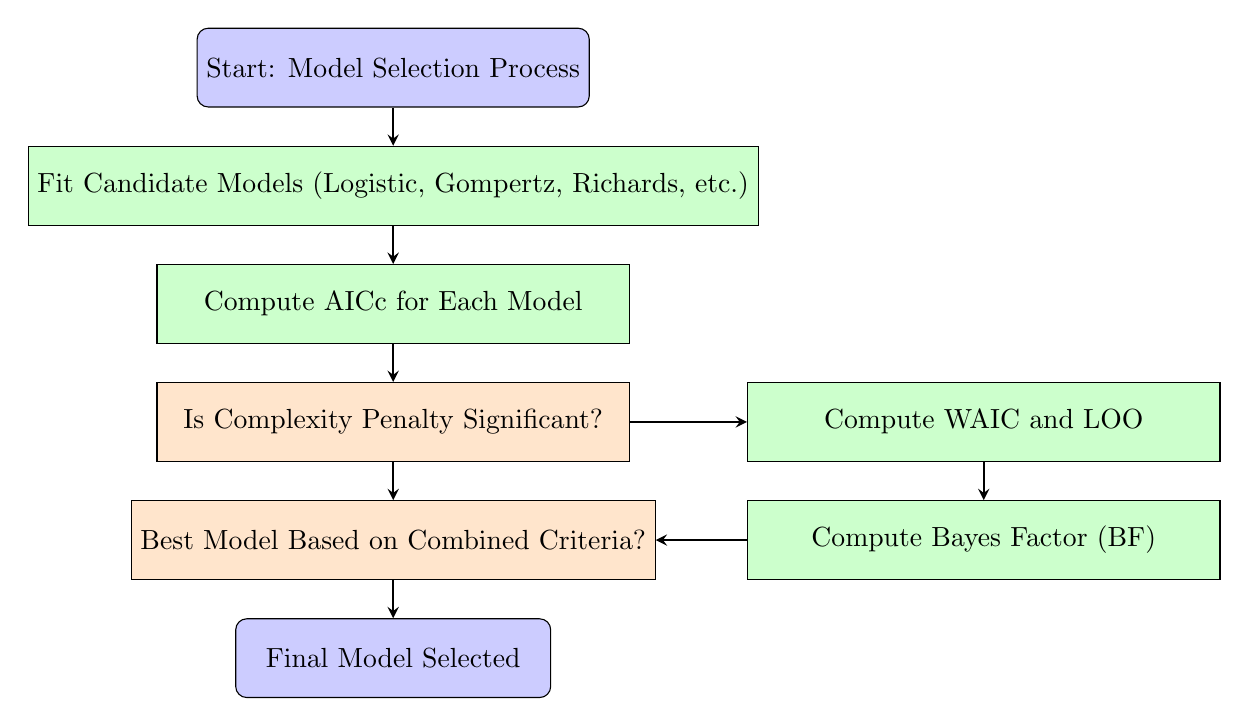
\begin{tikzpicture}[node distance=1.5cm]
    % Nodes
    \node (start) [startstop] {Start: Model Selection Process};
    \node (fitmodels) [process, below of=start] {Fit Candidate Models (Logistic, Gompertz, Richards, etc.)};
    \node (computeAIC) [process, below of=fitmodels] {Compute AICc for Each Model};
    \node (complexity) [decision, below of=computeAIC] {Is Complexity Penalty Significant?};
    \node (computeWAIC) [process, right of=complexity, xshift=6cm] {Compute WAIC and LOO};
    \node (computeBF) [process, below of=computeWAIC] {Compute Bayes Factor (BF)};
    \node (bestmodel) [decision, below of=complexity] {Best Model Based on Combined Criteria?};
    \node (finalmodel) [startstop, below of=bestmodel] {Final Model Selected};

    % Arrows
    \draw [arrow] (start) -- (fitmodels);
    \draw [arrow] (fitmodels) -- (computeAIC);
    \draw [arrow] (computeAIC) -- (complexity);
    \draw [arrow] (complexity.east) -- (computeWAIC.west);
    \draw [arrow] (computeWAIC) -- (computeBF);
    \draw [arrow] (computeBF.west) |- (bestmodel.east);
    \draw [arrow] (complexity.south) -- (bestmodel.north);
    \draw [arrow] (bestmodel.south) -- (finalmodel.north);
\end{tikzpicture}
\end{center}


